\chapter{Las capas electrónicas y la tabla periódica}\label{ch:g10:electron-shells}

El neón brilla con un color rojo anaranjado en un letrero; el sodio, un
\omterm{def:g9:periodic-table-first-look:metal}{metal} blando, se inflama en el agua; el cloro es un gas amarillo verdoso
y asfixiante. Sin embargo, sus \omterm{def:g7:atoms-and-molecules:atom}{átomos} solo se diferencian en uno o dos
\omterm{def:g9:inside-the-atom:proton}{protones}: el neón tiene 10, el sodio 11 y el cloro 17. ¿Por qué unos
vecinos de la \omterm{def:g9:periodic-table-first-look:periodic-table}{tabla periódica} se comportan de forma tan distinta,
mientras que el sodio y el potasio, alejados en \omterm{def:g9:inside-the-atom:atomic-number}{número atómico}, se
comportan de forma tan parecida? La respuesta está en cómo se disponen
los \omterm{def:g9:inside-the-atom:nucleus}{electrones} de un \omterm{def:g7:atoms-and-molecules:atom}{átomo}.

\begin{recall}
Un \omterm{def:g7:atoms-and-molecules:atom}{átomo} tiene $Z$ \omterm{def:g9:inside-the-atom:proton}{protones} en su \omterm{def:g9:inside-the-atom:nucleus}{núcleo} y, si es neutro, $Z$ \omterm{def:g9:inside-the-atom:nucleus}{electrones}
a su alrededor (\cref{ch:g9:inside-the-atom}). La \omterm{def:g9:periodic-table-first-look:periodic-table}{tabla periódica} ordena
los elementos según $Z$ en periodos (filas) y grupos (columnas); los
elementos de un grupo se comportan igual (\cref{ch:g9:periodic-table-first-look}).
Los \omterm{def:g7:atoms-and-molecules:atom}{átomos} ganan o pierden \omterm{def:g9:inside-the-atom:nucleus}{electrones} y se convierten en \omterm{def:g9:ions:ion}{iones}
(\cref{ch:g9:ions}).
\end{recall}

\section{La configuración electrónica}

\begin{definition}[Capas, subcapas y configuración electrónica]\label{def:g10:electron-shells:configuration}
Los \omterm{def:g9:inside-the-atom:nucleus}{electrones} de un \omterm{def:g7:atoms-and-molecules:atom}{átomo} se disponen en \emph{capas}\index{capa},
numeradas $n = 1, 2, 3, \ldots$ del \omterm{def:g9:inside-the-atom:nucleus}{núcleo} hacia fuera; cuanto mayor es
$n$, más lejos del \omterm{def:g9:inside-the-atom:nucleus}{núcleo} están los \omterm{def:g9:inside-the-atom:nucleus}{electrones} y menos fuertemente
retenidos. Cada capa se divide en \emph{subcapas}\index{subcapa}
designadas por una letra: la capa 1 tiene una subcapa s (1s), la capa 2
una subcapa s y una p (2s, 2p), la capa 3 tiene 3s y 3p (y 3d, que se
verá más adelante). Una subcapa s admite como mucho 2 \omterm{def:g9:inside-the-atom:nucleus}{electrones}, y una
subcapa p, como mucho 6. La
\emph{configuración electrónica}\index{configuracion electronica@configuración electrónica} de un
\omterm{def:g7:atoms-and-molecules:atom}{átomo} enumera sus subcapas ocupadas con su número de \omterm{def:g9:inside-the-atom:nucleus}{electrones} como
exponente: $1\mathrm{s}^2\,2\mathrm{s}^2\,2\mathrm{p}^4$ para el oxígeno.
\end{definition}

\begin{method}[Escribir una configuración electrónica, hasta $Z = 20$]\label{met:g10:electron-shells:write}
\begin{enumerate}
  \item Contar los \omterm{def:g9:inside-the-atom:nucleus}{electrones}: $Z$ para un \omterm{def:g7:atoms-and-molecules:atom}{átomo} neutro.
  \item Llenar las \omterm{def:g10:electron-shells:configuration}{subcapas} en este orden, cada una hasta su máximo
        antes de empezar la siguiente:
        \[
          1\mathrm{s} \to 2\mathrm{s} \to 2\mathrm{p} \to 3\mathrm{s} \to
          3\mathrm{p} \to 4\mathrm{s}.
        \]
  \item Comprobar que los exponentes suman el número de \omterm{def:g9:inside-the-atom:nucleus}{electrones}.
\end{enumerate}
Sodio, $Z = 11$: $1\mathrm{s}^2\,2\mathrm{s}^2\,2\mathrm{p}^6\,3\mathrm{s}^1$.
Cloro, $Z = 17$: $1\mathrm{s}^2\,2\mathrm{s}^2\,2\mathrm{p}^6\,3\mathrm{s}^2\,3\mathrm{p}^5$.
Calcio, $Z = 20$: $1\mathrm{s}^2\,2\mathrm{s}^2\,2\mathrm{p}^6\,3\mathrm{s}^2\,3\mathrm{p}^6\,4\mathrm{s}^2$.
\end{method}

\begin{omfigure}
\begin{tikzpicture}[font=\small, y=0.95cm]
  \draw[->, black!60] (-0.4,0) -- (-0.4,5.4) node[above, align=center, font=\footnotesize]
    {más lejos\\ del núcleo};
  \foreach \y/\lab/\n/\x in {0.3/1s/2/0.5, 1.3/2s/2/0.5, 1.9/2p/6/2.4, 3.0/3s/2/0.5,
      3.6/3p/6/2.4, 4.4/4s/2/0.5} {
    \foreach \k in {1,...,\n} \draw[omDef, fill=omDef!10] (\x+0.42*\k-0.42,\y) rectangle ++(0.36,0.36);
    \node[anchor=east] at (\x-0.05,\y+0.18) {\lab};
  }
  \node[anchor=west, font=\footnotesize] at (5.3,0.48) {capa 1: como mucho 2 electrones};
  \node[anchor=west, font=\footnotesize] at (5.3,1.7) {capa 2: $2 + 6 = 8$};
  \node[anchor=west, font=\footnotesize] at (5.3,3.4) {capa 3: $2 + 6 = 8$ (hasta $Z = 18$)};
  \node[anchor=west, font=\footnotesize] at (5.3,4.58) {la 4s se llena antes que la 3d};
\end{tikzpicture}

{\small El orden de llenado, hasta $Z = 20$. Cada casilla es un sitio para
un \omterm{def:g9:inside-the-atom:nucleus}{electrón}: una \omterm{def:g10:electron-shells:configuration}{subcapa} s tiene 2 sitios, y una \omterm{def:g10:electron-shells:configuration}{subcapa} p, 6.}
\end{omfigure}

\section{Los electrones de valencia}

\begin{definition}[Electrones de valencia y electrones internos]\label{def:g10:electron-shells:valence}
Los \omterm{def:g9:inside-the-atom:nucleus}{electrones} de la \omterm{def:g10:electron-shells:configuration}{capa} ocupada más externa (la capa de mayor $n$) son
los \emph{electrones de valencia}\index{electron de valencia@electrón de valencia}; los demás
son los \emph{electrones internos}\index{electron interno@electrón interno}. Solo los
\omterm{def:g9:inside-the-atom:nucleus}{electrones} de valencia intervienen en las \omterm{def:g7:chemical-reactions:reaction}{reacciones químicas}.
\end{definition}

\begin{example}[Contar los electrones de valencia]\label{ex:g10:electron-shells:count}
Oxígeno, $1\mathrm{s}^2\,2\mathrm{s}^2\,2\mathrm{p}^4$: \omterm{def:g10:electron-shells:configuration}{capa} externa $n =
2$, $2 + 4 = 6$ \omterm{def:g10:electron-shells:valence}{electrones de valencia}. Sodio, $\ldots 3\mathrm{s}^1$: 1
\omterm{def:g10:electron-shells:valence}{electrón de valencia}. Cloro, $\ldots 3\mathrm{s}^2\,3\mathrm{p}^5$: 7.
Neón, $1\mathrm{s}^2\,2\mathrm{s}^2\,2\mathrm{p}^6$: 8, una \omterm{def:g10:electron-shells:configuration}{capa} completa.
\end{example}

\section{La tabla reconstruida a partir de las configuraciones}

\begin{proposition}[Periodo y grupo a partir de la configuración]\label{prop:g10:electron-shells:table}
Para los elementos hasta $Z = 20$:
\begin{itemize}
  \item el periodo de un elemento es el número $n$ de su \omterm{def:g10:electron-shells:configuration}{capa} externa;
  \item los elementos de un mismo grupo tienen el mismo número de
        \omterm{def:g10:electron-shells:valence}{electrones de valencia}: uno en el \omterm{def:g9:periodic-table-first-look:period}{grupo} 1, dos en el \omterm{def:g9:periodic-table-first-look:period}{grupo} 2, de
        tres a ocho en los \omterm{def:g9:periodic-table-first-look:period}{grupos} 13 a 18 (el helio, con 2, es una
        excepción).
\end{itemize}
Las dos columnas de la izquierda, donde los últimos \omterm{def:g9:inside-the-atom:nucleus}{electrones} entran en
una \omterm{def:g10:electron-shells:configuration}{subcapa} s, forman el bloque s; los \omterm{def:g9:periodic-table-first-look:period}{grupos} 13 a 18 forman el bloque
p.
\end{proposition}

\begin{omfigure}
\omperiodictable[upto=20, f block=false, cell=0.86cm, colour=blocks, legend=true,
  values={H/1,He/2,Li/2.1,Be/2.2,B/2.3,C/2.4,N/2.5,O/2.6,F/2.7,Ne/2.8,
    Na/2.8.1,Mg/2.8.2,Al/2.8.3,Si/2.8.4,P/2.8.5,S/2.8.6,Cl/2.8.7,Ar/2.8.8,
    K/2.8.8.1,Ca/2.8.8.2}]

{\small Los veinte primeros elementos, con el número de \omterm{def:g9:inside-the-atom:nucleus}{electrones} de
cada capa debajo del símbolo ($2.8.1$ para el sodio: 2 en la \omterm{def:g10:electron-shells:configuration}{capa} 1, 8
en la \omterm{def:g10:electron-shells:configuration}{capa} 2 y 1 en la \omterm{def:g10:electron-shells:configuration}{capa} 3). Los colores marcan los bloques s y p.}
\end{omfigure}

\section{Las familias}

\begin{definition}[Familias químicas]\label{def:g10:electron-shells:family}
Una \emph{familia química}\index{familia quimica@familia química} es un grupo de la
\omterm{def:g9:periodic-table-first-look:periodic-table}{tabla periódica} cuyos elementos comparten sus principales propiedades
químicas. Se nombran tres familias: los
\emph{metales alcalinos}\index{metal alcalino} (el \omterm{def:g9:periodic-table-first-look:period}{grupo} 1 salvo el
hidrógeno: litio, sodio, potasio\dots), \omterm{def:g9:periodic-table-first-look:metal}{metales} blandos que reaccionan
con fuerza con el agua; los \emph{halógenos}\index{halogeno@halógeno} (\omterm{def:g9:periodic-table-first-look:period}{grupo} 17:
flúor, cloro, bromo, yodo), \omterm{def:g9:periodic-table-first-look:metal}{no metales} de color y reactivos; y los
\emph{gases nobles}\index{gas noble} (\omterm{def:g9:periodic-table-first-look:period}{grupo} 18: helio, neón,
argón\dots), que casi no reaccionan con nada.
\end{definition}

\begin{proposition}[Por qué una familia se comporta igual]\label{prop:g10:electron-shells:why}
Los elementos de una familia tienen el mismo número de \omterm{def:g10:electron-shells:valence}{electrones de
valencia}, y la química es cosa de los \omterm{def:g10:electron-shells:valence}{electrones de valencia}: el litio,
el sodio y el potasio tienen uno; los \omterm{def:g10:electron-shells:family}{halógenos}, siete; los \omterm{def:g10:electron-shells:family}{gases
nobles}, una \omterm{def:g10:electron-shells:configuration}{capa} externa completa.
\end{proposition}

\begin{omfigure}
\omperiodictable[colour=families, legend=true, cell=0.86cm, f block=false]

{\small Familias de la \omterm{def:g9:periodic-table-first-look:periodic-table}{tabla periódica}: \omterm{def:g10:electron-shells:family}{metales alcalinos}, \omterm{def:g9:periodic-table-first-look:metal}{metales}
alcalinotérreos (\omterm{def:g9:periodic-table-first-look:period}{grupo} 2), \omterm{def:g10:electron-shells:family}{halógenos} y \omterm{def:g10:electron-shells:family}{gases nobles}.}
\end{omfigure}

\begin{omfigure}
\begin{minipage}[b]{0.48\linewidth}\centering
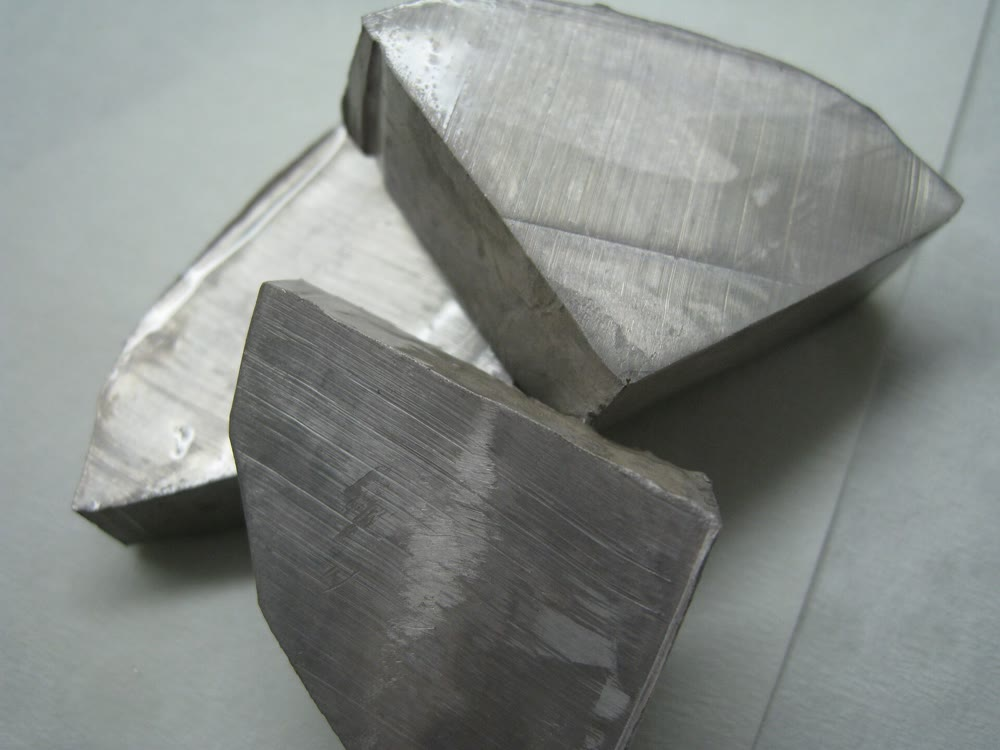
\includegraphics[width=\linewidth,height=4.4cm,keepaspectratio]{images/book1/sodium.jpg}

{\small El sodio, un \omterm{def:g10:electron-shells:family}{metal alcalino}, cortado con un cuchillo: blando y
plateado cuando está recién cortado, se empaña enseguida al \omterm{def:g4:air-a-mixture-of-gases:air}{aire}. Foto:
Dnn87, CC BY-SA 3.0.}
\end{minipage}\hfill
\begin{minipage}[b]{0.48\linewidth}\centering
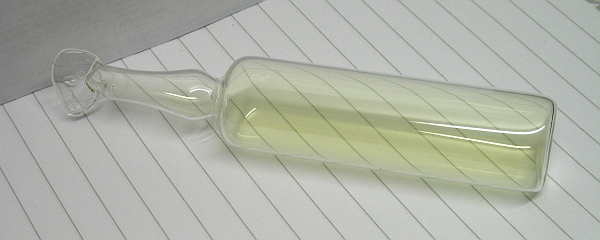
\includegraphics[width=\linewidth,height=4.4cm,keepaspectratio]{images/book1/chlorine-ampoule.jpg}

{\small El cloro, un \omterm{def:g10:electron-shells:family}{halógeno}: un gas amarillo verdoso, aquí encerrado en
una ampolla de vidrio. Foto: W.~Oelen, CC BY-SA 3.0.}
\end{minipage}
\end{omfigure}

\begin{inthelab}[Sodio en agua]
Detrás de una pantalla, el profesor echa un trozo de sodio del tamaño de
un grano de arroz en un barreño grande de agua. Flota, se funde en una
bolita brillante y corre de un lado a otro, burbujeando, hasta que
desaparece; el gas que se desprende es hidrógeno, y el agua que queda es
básica.
\end{inthelab}

\begin{safety}{\ghs[0.75cm]{GHS02}\ghs[0.75cm]{GHS05}\quad\ghs[0.75cm]{GHS03}\ghs[0.75cm]{GHS06}}
% ledger: ghs:Na, ghs:Cl2
Sodio: con el agua desprende hidrógeno inflamable (GHS02), provoca
quemaduras graves (GHS05). Cloro: un gas comburente (GHS03), tóxico en
caso de inhalación (GHS06), además de irritante y muy tóxico para los
organismos acuáticos. Los dos los manipula solo el profesor.
\end{safety}

\section{Los iones estables y la regla de los gases nobles}

\begin{definition}[Reglas del dúo y del octeto]\label{def:g10:electron-shells:octet}
Los \omterm{def:g10:electron-shells:family}{gases nobles}, con una \omterm{def:g10:electron-shells:configuration}{capa} externa completa, casi no reaccionan: su
configuración es especialmente estable. Cuando los \omterm{def:g7:atoms-and-molecules:atom}{átomos} de los
primeros elementos forman \omterm{def:g9:ions:ion}{iones}, ganan o pierden \omterm{def:g9:inside-the-atom:nucleus}{electrones} para
alcanzar la configuración del \omterm{def:g10:electron-shells:family}{gas noble} más cercano: dos \omterm{def:g9:inside-the-atom:nucleus}{electrones} en
la \omterm{def:g10:electron-shells:configuration}{capa} 1, como el helio, para los \omterm{def:g7:atoms-and-molecules:atom}{átomos} más ligeros (la
\emph{regla del dúo}\index{regla del duo@regla del dúo}), y ocho \omterm{def:g9:inside-the-atom:nucleus}{electrones} en la \omterm{def:g10:electron-shells:configuration}{capa}
externa, como el neón o el argón, para los demás (la
\emph{regla del octeto}\index{regla del octeto}).
\end{definition}

\begin{example}[Iones que predice la regla]\label{ex:g10:electron-shells:ions}
El sodio, $2.8.1$, pierde su único \omterm{def:g10:electron-shells:valence}{electrón de valencia}: \ce{Na+},
$2.8$, como el neón. El magnesio, $2.8.2$, pierde dos: \ce{Mg^{2+}}. El
aluminio, $2.8.3$, pierde tres: \ce{Al^{3+}}. El cloro, $2.8.7$, gana
uno: \ce{Cl-}, $2.8.8$, como el argón. El oxígeno, $2.6$, gana dos:
\ce{O^{2-}}. El azufre, $2.8.6$: \ce{S^{2-}}. El litio, $2.1$, pierde
uno y se queda con $2$, como el helio: \ce{Li+}.
\end{example}

\begin{omfigure}
\begin{tikzpicture}[font=\small]
  \foreach \x/\nm/\cfg/\col in {0/{Na}/{$1\mathrm{s}^2\,2\mathrm{s}^2\,2\mathrm{p}^6\,3\mathrm{s}^1$}/omDef,
      5.8/{\ce{Na+}}/{$1\mathrm{s}^2\,2\mathrm{s}^2\,2\mathrm{p}^6$}/omProp,
      11.0/{Ne}/{$1\mathrm{s}^2\,2\mathrm{s}^2\,2\mathrm{p}^6$}/gray} {
    \node[draw=\col, fill=\col!6, rounded corners=2pt, align=center, text width=3.4cm]
      at (\x,0) {\textbf{\nm}\\ \cfg};
  }
  \draw[->, thick, omProp] (2.0,0) -- (3.8,0) node[midway, above, font=\footnotesize] {pierde 1 \ce{e-}};
  \node at (8.4,0) {$=$};
  \node[font=\footnotesize, align=center] at (8.4,-0.75) {la misma\\ configuración};
\end{tikzpicture}

{\small El \omterm{def:g9:ions:ion}{ion} sodio tiene la configuración del neón, el \omterm{def:g10:electron-shells:family}{gas noble} más
cercano.}
\end{omfigure}

\begin{remark}[Límites de la regla]\label{rem:g10:electron-shells:limits}
La regla funciona bien para los veinte primeros elementos y sus \omterm{def:g9:ions:ion}{iones}
sencillos. Muchos elementos, como el hierro (\ce{Fe^{2+}} y
\ce{Fe^{3+}}), no la cumplen; las razones, y una descripción mejor de
los \omterm{def:g9:inside-the-atom:nucleus}{electrones}, se dan en el volumen del primer año universitario.
\end{remark}

\section{Ejercicios}

\begin{exercise}[$\star$]\label{exo:g10:electron-shells:1}
Escribe las \omterm{def:g10:electron-shells:configuration}{configuraciones electrónicas} del carbono ($Z = 6$), el
nitrógeno ($Z = 7$) y el magnesio ($Z = 12$).
\end{exercise}

\begin{exercise}[$\star$]\label{exo:g10:electron-shells:2}
¿Cuántos \omterm{def:g10:electron-shells:valence}{electrones de valencia} tienen el carbono, el nitrógeno y el
magnesio?
\end{exercise}

\begin{exercise}[$\star$]\label{exo:g10:electron-shells:3}
¿En qué periodo y en qué grupo está el elemento de configuración
$1\mathrm{s}^2\,2\mathrm{s}^2\,2\mathrm{p}^6\,3\mathrm{s}^2\,3\mathrm{p}^3$?
\end{exercise}

\begin{exercise}[$\star$]\label{exo:g10:electron-shells:4}
Nombra las tres familias de este capítulo y da dos elementos de cada una.
\end{exercise}

\begin{exercise}[$\star$]\label{exo:g10:electron-shells:5}
Enuncia la \omterm{def:g10:electron-shells:octet}{regla del octeto}.
\end{exercise}

\begin{exercise}[$\star\star$]\label{exo:g10:electron-shells:6}
Con la regla de los \omterm{def:g10:electron-shells:family}{gases nobles}, da el \omterm{def:g9:ions:ion}{ion} que forma el potasio
($Z = 19$) y el que forma el flúor ($Z = 9$), con sus configuraciones.
\end{exercise}

\begin{exercise}[$\star\star$]\label{exo:g10:electron-shells:7}
Un elemento tiene 2 \omterm{def:g9:inside-the-atom:nucleus}{electrones} en su tercera capa, y la tercera capa es
su \omterm{def:g10:electron-shells:configuration}{capa} externa. Da su configuración, su \omterm{def:g9:inside-the-atom:atomic-number}{número atómico} y su nombre.
\end{exercise}

\begin{exercise}[$\star\star$]\label{exo:g10:electron-shells:8}
Con los \omterm{def:g9:ions:ion}{iones} estables, escribe la fórmula del \omterm{def:g9:ions:ionic-compound}{compuesto iónico} formado
por el magnesio y el cloro, y después la del formado por el aluminio y
el oxígeno.
\end{exercise}

\begin{exercise}[$\star\star$]\label{exo:g10:electron-shells:9}
Mira la tabla de los veinte primeros elementos. ¿Qué elementos tienen el
mismo número de \omterm{def:g10:electron-shells:valence}{electrones de valencia} que el oxígeno?
\end{exercise}

\begin{exercise}[$\star\star$]\label{exo:g10:electron-shells:10}
¿Por qué el neón, a diferencia del sodio y del cloro, no forma \omterm{def:g9:ions:ion}{iones} en
las \omterm{def:g7:chemical-reactions:reaction}{reacciones químicas}?
\end{exercise}

\begin{exercise}[$\star\star$]\label{exo:g10:electron-shells:11}
El \omterm{def:g9:ions:ion}{ion} \ce{X^{2+}} tiene la configuración del argón. Halla $X$.
\end{exercise}

\begin{exercise}[$\star\star\star$]\label{exo:g10:electron-shells:12}
El helio tiene 2 \omterm{def:g10:electron-shells:valence}{electrones de valencia}, pero está en el \omterm{def:g9:periodic-table-first-look:period}{grupo} 18 y no
en el \omterm{def:g9:periodic-table-first-look:period}{grupo} 2. Explícalo con su configuración.
\end{exercise}

\begin{exercise}[$\star\star\star$]\label{exo:g10:electron-shells:13}
El potasio reacciona con el agua todavía más violentamente que el sodio.
A partir de la distancia del \omterm{def:g10:electron-shells:valence}{electrón de valencia} al \omterm{def:g9:inside-the-atom:nucleus}{núcleo}, propón una
explicación.
\end{exercise}

\begin{exercise}[$\star\star\star$]\label{exo:g10:electron-shells:14}
Da las configuraciones de \ce{S^{2-}}, \ce{Cl-}, \ce{K+} y
\ce{Ca^{2+}}. ¿Qué tienen en común?
\end{exercise}

\begin{exercise}[$\star\star\star$]\label{exo:g10:electron-shells:15}
Un elemento del periodo 3 forma el \omterm{def:g9:ions:ion}{ion} \ce{Y^{3-}}. Halla su grupo, su
configuración y su nombre.
\end{exercise}

\section{Problema: Rubí, zafiro y corindón}

\begin{problem}[{Problema de fin de semana --- los electrones que hay
detrás de una piedra preciosa: de dos configuraciones al número de
electrones transferidos en un gramo}]
\label{pb:g10:electron-shells:1}
Los rubíes y los zafiros son variedades preciosas del corindón, un
\omterm{def:g9:ions:ionic-compound}{compuesto iónico} de aluminio y oxígeno; una traza de otros \omterm{def:g9:periodic-table-first-look:metal}{metales} les da
su color. El corindón es tan duro que raya casi cualquier cosa, y el
corindón en polvo se usa para pulir lentes. Toma como masa de un \omterm{def:g9:inside-the-atom:proton}{nucleón}
\qty{1.67e-27}{kg}; el aluminio~27 tiene 27 \omterm{def:g9:inside-the-atom:proton}{nucleones}, y el oxígeno~16,
16.

\medskip
\noindent\textbf{Parte I --- Los \omterm{def:g7:atoms-and-molecules:atom}{átomos}.}
\begin{enumerate}
  \item Da el número de \omterm{def:g9:inside-the-atom:proton}{protones} y de \omterm{def:g9:inside-the-atom:nucleus}{electrones} de un \omterm{def:g7:atoms-and-molecules:atom}{átomo} de aluminio
        ($Z = 13$) y de un \omterm{def:g7:atoms-and-molecules:atom}{átomo} de oxígeno ($Z = 8$).
  \item Escribe sus \omterm{def:g10:electron-shells:configuration}{configuraciones electrónicas}.
  \item ¿Cuántos \omterm{def:g10:electron-shells:valence}{electrones de valencia} tiene cada uno? ¿En qué periodo
        y en qué grupo está cada uno?
  \item ¿El aluminio es un \omterm{def:g9:periodic-table-first-look:metal}{metal} o un \omterm{def:g9:periodic-table-first-look:metal}{no metal}? ¿Y el oxígeno?
\end{enumerate}

\medskip
\noindent\textbf{Parte II --- Los \omterm{def:g9:ions:ion}{iones}.}
\begin{enumerate}[resume]
  \item Con la \omterm{def:g10:electron-shells:octet}{regla del octeto}, ¿qué \omterm{def:g9:ions:ion}{ion} forma el aluminio? Escribe su
        configuración.
  \item ¿Qué \omterm{def:g9:ions:ion}{ion} forma el oxígeno? Escribe su configuración.
  \item ¿Qué \omterm{def:g10:electron-shells:family}{gas noble} tiene la misma configuración que los dos \omterm{def:g9:ions:ion}{iones}?
  \item ¿Cuántos \omterm{def:g9:inside-the-atom:nucleus}{electrones} pierde un \omterm{def:g7:atoms-and-molecules:atom}{átomo} de aluminio, y cuántos gana
        un \omterm{def:g7:atoms-and-molecules:atom}{átomo} de oxígeno?
\end{enumerate}

\medskip
\noindent\textbf{Parte III --- La fórmula.}
\begin{enumerate}[resume]
  \item Halla la fórmula del corindón, el compuesto neutro de estos
        \omterm{def:g9:ions:ion}{iones}.
  \item En una unidad fórmula, ¿cuántos \omterm{def:g9:inside-the-atom:nucleus}{electrones} pierden los \omterm{def:g7:atoms-and-molecules:atom}{átomos} de
        aluminio? ¿Cuántos ganan los \omterm{def:g7:atoms-and-molecules:atom}{átomos} de oxígeno?
  \item ¿Por qué deben ser iguales estos dos números?
  \item Un rubí contiene una traza de \omterm{def:g9:ions:ion}{iones} cromo \ce{Cr^{3+}} en lugar
        de algunos \ce{Al^{3+}}. ¿Por qué un \omterm{def:g9:ions:ion}{ion} \ce{Cr^{3+}} puede
        ocupar el lugar de un \omterm{def:g9:ions:ion}{ion} \ce{Al^{3+}} sin alterar las cargas?
\end{enumerate}

\medskip
\noindent\textbf{Parte IV --- Un gramo de corindón.}
\begin{enumerate}[resume]
  \item ¿Cuántos \omterm{def:g9:inside-the-atom:proton}{nucleones} hay en una unidad fórmula de corindón?
  \item Calcula la masa de una unidad fórmula (despreciando los
        \omterm{def:g9:inside-the-atom:nucleus}{electrones}).
  \item ¿Cuántas unidades fórmula hay en \qty{1}{g} de corindón?
  \item ¿Cuántos \omterm{def:g9:ions:ion}{iones} \ce{Al^{3+}} y cuántos \omterm{def:g9:ions:ion}{iones} \ce{O^{2-}} son?
  \item ¿Por qué se pueden despreciar los \omterm{def:g9:inside-the-atom:nucleus}{electrones} en la pregunta 14?
  \item ¿Cuántos \omterm{def:g9:inside-the-atom:nucleus}{electrones} se transfirieron del aluminio al oxígeno para
        formar \qty{1}{g} de corindón?
\end{enumerate}
\end{problem}
